\chapter{Equation of State, Radiation, and Vacuum Energy}

These companion notes follow Leonard Susskind's fifth lecture in the Cosmology course, with curation support by LazyingArt LLC and Video2Book. The lecture begins by stepping back to the main cosmological question, the time history of the scale factor \(a(t)\), and then asks what extra input is needed to turn the Friedmann equation into actual cosmological histories. The answer is the equation of state. We will first derive the general scaling law for the energy density, then compute \(w=\tfrac13\) for radiation from a photon box, and finally turn to vacuum energy, where the equation of state becomes \(w=-1\) and the dynamics of the universe change qualitatively.

\section{Review: The Scale Factor and the Missing Input}

The overriding question in these notes is the same question that has been running through the course from the beginning: what is the history of the universe? In the homogeneous and isotropic approximation, that question reduces to one central function, the scale factor \(a(t)\). If we know how \(a(t)\) evolves, then we know a great deal about the large-scale history of the universe.

Two simple models have already appeared. In a matter-dominated universe,
\begin{equation}
a(t)\propto t^{2/3},
\end{equation}
while in a radiation-dominated universe,
\begin{equation}
a(t)\propto t^{1/2}.
\end{equation}
Neither law is exact for all times. At early times radiation is the better approximation; at late times matter is the better approximation. But the point of the review is not only to recall these exponents. It is to put back on the table the quantity that distinguishes the two cases: the energy density \(\rho\).

\begin{figure}[h]
\centering

\includegraphics[width=0.72\textwidth]{lecture_05_figure_02.png}
\caption{Reviewed scale-factor laws with newly introduced energy-density notation.}
\end{figure}

The lecture's pivot is explicit. The equation of state is what tells us how the energy density on the right-hand side of the Friedmann equation changes as the universe expands. For the two cases just reviewed, the corresponding density laws are
\begin{equation}
\rho_{\text{matter}}=\frac{\rho_0}{a^3},
\qquad
\rho_{\text{rad}}=\frac{\rho_0}{a^4}.
\end{equation}
The first of these is easy to understand at sight: matter simply dilutes with the volume, and volume scales like \(a^3\). Radiation is more subtle. The density does not merely fall like \(a^{-3}\); there is one extra power of \(a\). The lecture now asks where that extra power comes from, and more generally what relation between pressure and energy density produces a given scaling law for \(\rho\).

\section{From the Equation of State to the Density-Scaling Law}

In cosmology we make a simplifying assumption that covers many important cases:
\begin{equation}
P=w\rho.
\end{equation}
The parameter \(w\) characterizes the fluid. On the lecture board the same symbol is written as an uppercase \(W\), but we will use the conventional lowercase \(w\).

\begin{figure}[h]
\centering

\includegraphics[width=0.86\textwidth]{lecture_05_figure_03.png}
\caption{Equation of state and thermodynamic box argument.}
\end{figure}

The lecture does not simply assert the familiar formula \(\rho\propto a^{-3(1+w)}\). Instead it rebuilds it from a box argument. We imagine a gas in a box, and we move one wall slightly outward. If the wall has area \(A\) and is displaced by \(dx\), then the change in volume is
\begin{equation}
dV=A\,dx.
\end{equation}
The force on the wall is \(P A\), so the work done by the gas is \(P A\,dx=P\,dV\). Since the gas does the work, the energy remaining inside the box decreases:
\begin{equation}
dE=-P\,dV.
\end{equation}

\begin{figure}[h]
\centering
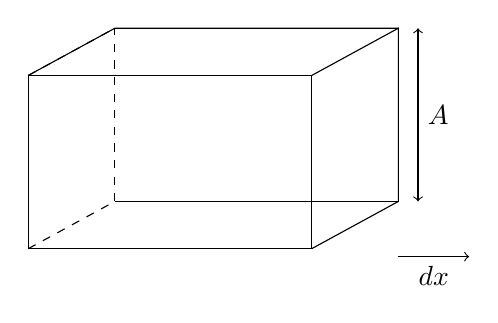
\begin{tikzpicture}[scale=1.0]
\draw (0,0) -- (3.6,0) -- (3.6,2.2) -- (0,2.2) -- cycle;
\draw (3.6,0) -- (4.7,0.6) -- (4.7,2.8) -- (3.6,2.2);
\draw (0,2.2) -- (1.1,2.8) -- (4.7,2.8);
\draw (1.1,0.6) -- (4.7,0.6);
\draw[dashed] (0,0) -- (1.1,0.6);
\draw[dashed] (0,2.2) -- (1.1,2.8);
\draw[dashed] (1.1,0.6) -- (1.1,2.8);
\draw[<->] (4.95,0.6) -- (4.95,2.8);
\node[right] at (4.95,1.7) {\(A\)};
\draw[->] (4.7,-0.1) -- (5.6,-0.1);
\node[below] at (5.15,-0.1) {\(dx\)};
\end{tikzpicture}
\caption{A clean redraw of the thermodynamic box used in the lecture.}
\end{figure}

Now we use the fact that the total energy in the box is
\begin{equation}
E=\rho V.
\end{equation}
Differentiating gives
\begin{equation}
d(\rho V)=\rho\,dV+V\,d\rho.
\end{equation}
Substituting this into the work relation,
\begin{equation}
\rho\,dV+V\,d\rho=-P\,dV.
\end{equation}
If we now impose the equation of state \(P=w\rho\), then the \(\rho\,dV\) term on the left and the \(w\rho\,dV\) term on the right combine to give
\begin{equation}
V\,d\rho=-(1+w)\rho\,dV.
\end{equation}
Dividing by \(\rho V\), we obtain the separated differential equation
\begin{equation}
\frac{d\rho}{\rho}=-(1+w)\frac{dV}{V}.
\end{equation}

\begin{figure}[h]
\centering

\includegraphics[width=0.78\textwidth]{lecture_05_figure_04.png}
\caption{Logarithmic integration of the density-volume relation.}
\end{figure}

This is the point where the board in the lecture shows the separation clearly and begins the logarithmic line with \(\log\rho=\). The fully integrated form is the natural standard completion of that board state:
\begin{equation}
d(\log \rho)=-(1+w)\,d(\log V),
\end{equation}
and therefore
\begin{equation}
\log \rho=-(1+w)\log V+\text{const.}
\end{equation}
Exponentiating,
\begin{equation}
\rho\propto V^{-(1+w)}.
\end{equation}

For cosmology we imagine not merely a one-sided deformation of the box, but isotropic expansion. Then the volume of a comoving chunk of space scales as
\begin{equation}
V\propto a^3.
\end{equation}
So the density law becomes
\begin{equation}
\rho\propto a^{-3(1+w)}.
\end{equation}
This is the famous equation the lecture has been walking toward, but it is important that it arrive only after the thermodynamic argument has made it intelligible.

\section{First Applications: Matter and Radiation}

The opening review now closes back on itself. Matter domination corresponds to nonrelativistic particles. Their energy is dominated by rest mass, while the pressure generated by particles striking the wall depends on their comparatively small velocities. Thus pressure is negligible compared to energy density, and we take
\begin{equation}
w=0.
\end{equation}
Plugging this into the general law gives
\begin{equation}
\rho\propto a^{-3},
\end{equation}
which is exactly the matter-dilution law we reviewed at the beginning.

Radiation is different. For radiation the lecture announces the answer first and then derives it:
\begin{equation}
w=\frac13.
\end{equation}
If this is true, then
\begin{equation}
\rho\propto a^{-3(1+1/3)}=a^{-4}.
\end{equation}
So the extra inverse power of \(a\) in radiation domination is not an independent assumption. It is the consequence of a different equation of state. The next task is therefore clear: we must explain why radiation has \(w=\tfrac13\).

\section{Why Radiation Has \(w=\frac13\)}

Radiation means massless particles, and for present purposes we think of those particles as photons. The distinguishing feature is that photons move with the speed of light. Therefore the pressure they exert cannot be understood in the same way as pressure from slow nonrelativistic particles.

We begin by introducing the notation used in the lecture. Let \(\epsilon\) denote the energy per photon, and let \(\vec{\pi}\) denote the photon momentum vector. The symbol \(p\) is avoided because \(P\) is already being used for pressure. For a massless particle,
\begin{equation}
\epsilon = c\,\pi,
\end{equation}
where \(\pi=|\vec{\pi}|\). In the units used throughout the course, \(c=1\), so
\begin{equation}
\epsilon=\pi.
\end{equation}
If \(\nu\) is the photon number density, then the energy density is
\begin{equation}
\rho=\epsilon\,\nu.
\end{equation}

Now consider a wall of the box, and let the \(x\)-axis be normal to that wall. A photon moving at angle \(\theta\) relative to the normal can hit the wall during a short time interval \(\Delta t\) only if it starts inside a thin slab of thickness
\begin{equation}
\Delta x=\Delta t\cos\theta.
\end{equation}
When such a photon reflects, its normal momentum component reverses sign. The change in normal momentum is therefore
\begin{equation}
\Delta \pi_x = 2\epsilon \cos\theta.
\end{equation}
The force contributed by one hit is \(\Delta \pi_x/\Delta t\). The number of photons in the slab is \(\nu A \Delta x\), but only half of them are moving toward the wall, so the number of relevant photons is \(\tfrac12 \nu A \Delta x\). Dividing the total force by the wall area \(A\), we find
\begin{align}
P(\theta)
&=
\frac{1}{A}
\left(\frac{2\epsilon\cos\theta}{\Delta t}\right)
\left(\frac12 \nu A \Delta x\right) \\
&=
\epsilon \nu \cos\theta \frac{\Delta x}{\Delta t} \\
&=
\epsilon \nu \cos^2\theta \\
&=
\rho \cos^2\theta.
\end{align}
At this stage the pressure still seems to depend on angle, but that is only because we have computed the contribution from photons traveling in one direction.

\begin{figure}[h]
\centering
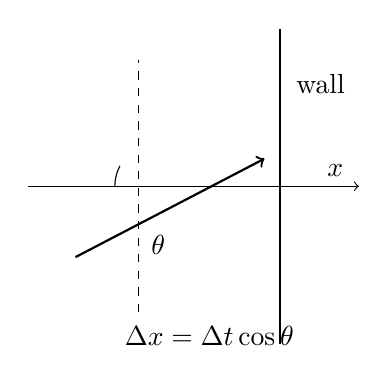
\begin{tikzpicture}[scale=1.0]
\draw[thick] (0,0) -- (0,4);
\draw[->] (-3.2,2) -- (1.0,2);
\node[above] at (0.7,2) {\(x\)};
\draw[dashed] (-1.8,0.4) -- (-1.8,3.6);
\node[below] at (-0.9,0.35) {\(\Delta x=\Delta t\cos\theta\)};
\draw[->,thick] (-2.6,1.1) -- (-0.2,2.35);
\node[below] at (-1.55,1.5) {\(\theta\)};
\draw ( -2.1,2 ) arc[start angle=180,end angle=152,radius=0.55];
\node[right] at (0.08,3.3) {wall};
\end{tikzpicture}
\caption{Transcript-backed reconstruction of the photon-pressure geometry.}
\end{figure}

The remaining step is purely geometric. Let \(\mathbf n=(n_x,n_y,n_z)\) be the unit vector in the direction of motion of a photon. Then \(n_x=\cos\theta\), and
\begin{equation}
n_x^2+n_y^2+n_z^2=1.
\end{equation}
In an isotropic gas, the averages of \(n_x^2\), \(n_y^2\), and \(n_z^2\) are equal. Averaging the identity above,
\begin{equation}
\langle n_x^2\rangle+\langle n_y^2\rangle+\langle n_z^2\rangle=1,
\end{equation}
so isotropy implies
\begin{equation}
\langle n_x^2\rangle=\langle \cos^2\theta\rangle=\frac13.
\end{equation}
Therefore the averaged pressure is
\begin{equation}
P=\rho\langle \cos^2\theta\rangle=\frac{\rho}{3}.
\end{equation}
So the equation of state for radiation is
\begin{equation}
P=\frac13\rho,
\qquad
w=\frac13.
\end{equation}

\subsection{Question \& Answer}

\paragraph{Do we need all photons to have the same energy?} No. The equal-energy assumption is only a convenience. The argument may be carried out energy band by energy band, and each band separately obeys \(P=\rho/3\). Summing the contributions preserves the same equation of state.

\paragraph{What if the walls absorb instead of reflect?} The same answer survives. A black wall that absorbs and re-emits photons in thermal equilibrium gives the same net momentum balance. In cosmology there are of course no literal walls in space; the box is a bookkeeping device. What matters is local momentum flow across an imagined surface, and that balance is the same.

\paragraph{Do quantum statistics change the answer?} Not at the level relevant here. The lecture is explicit that quantum statistics do not alter the result \(P=\rho/3\).

\paragraph{What about photon-photon scattering?} In principle it can modify the equation of state, but only very slightly under ordinary cosmological conditions. At sufficiently high temperatures new processes can occur, such as pair production, and then the simple radiation equation of state can change. That lies beyond the approximation being used here.

\paragraph{What happened to the wall area?} The lecture itself pauses over this point. The intermediate calculation first gives the total force; only after dividing by the area do we obtain the pressure. The area cancels out in the final formula, as it should.

\section{Negative Pressure and Vacuum Energy}

Up to this point pressure has come from particles bouncing around and striking the boundary of a box. That makes positive pressure feel natural. The lecture now raises the next conceptual obstacle: can pressure be negative? The answer is yes, and the simplest way to see it is to think of negative pressure as tension.

In a one-dimensional world, a box is just an interval. If particles bounce between the two ends, they push the ends outward and produce positive pressure. But now imagine replacing those particles by a spring stretched between the two ends. When we pull the ends apart, the spring pulls back inward. That is not outward push but inward pull. In other words, it is tension, and tension is the one-dimensional analog of negative pressure.

\begin{figure}[h]
\centering
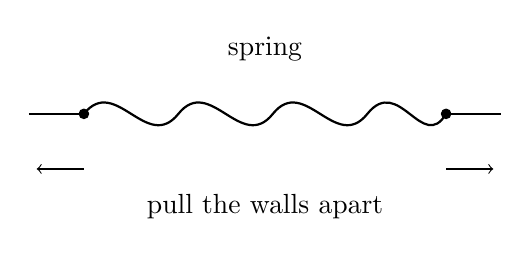
\begin{tikzpicture}[scale=1.0]
\draw[thick] (-3,0) -- (-2.3,0);
\draw[thick] (2.3,0) -- (3,0);
\draw[fill] (-2.3,0) circle (0.06);
\draw[fill] (2.3,0) circle (0.06);
\draw[thick] (-2.3,0)
.. controls (-1.9,0.5) and (-1.5,-0.5) .. (-1.1,0)
.. controls (-0.7,0.5) and (-0.3,-0.5) .. (0.1,0)
.. controls (0.5,0.5) and (0.9,-0.5) .. (1.3,0)
.. controls (1.7,0.5) and (2.0,-0.5) .. (2.3,0);
\draw[->] (-2.3,-0.7) -- (-2.9,-0.7);
\draw[->] (2.3,-0.7) -- (2.9,-0.7);
\node[below] at (0,-0.9) {pull the walls apart};
\node[above] at (0,0.55) {spring};
\end{tikzpicture}
\caption{A one-dimensional spring as an analogy for negative pressure.}
\end{figure}

This also changes the sign of the work relation in an instructive way. For ordinary positive pressure, increasing the size of the box lowers the energy stored inside: the system does work on the outside. For tension, increasing the size of the box stores more energy in the stretched system. So negative pressure is not an algebraic curiosity. It is physically familiar once we stop thinking only in terms of dilute particles bouncing off walls.

\subsection{Question \& Answer}

\paragraph{How can pressure be negative if the energy density is positive?} The spring picture answers precisely this. Energy can be stored in a configuration that pulls inward rather than pushes outward. Then \(P<0\) while \(\rho>0\), and so the equation-of-state parameter \(w=P/\rho\) is negative.

\paragraph{Is this central or peripheral?} It is central. The lecture stresses that if negative pressure were only a mathematical oddity it would not be worth dwelling on. It matters because the most important new fluid in modern cosmology, vacuum energy, behaves this way.

We now pass from the spring analogy to the actual cosmological example. Vacuum energy is the energy density of empty space itself. Whatever its microscopic origin may be, the defining macroscopic property is simple: the vacuum energy density does not dilute when we change the size of the box. It is a fixed property of empty space. We therefore write
\begin{equation}
\rho=\rho_0=\text{const.}
\end{equation}
If a box of volume \(V\) contains only vacuum energy, then
\begin{equation}
E=\rho_0 V.
\end{equation}
It is convenient to introduce a rescaled version of \(\rho_0\),
\begin{equation}
\Lambda=\frac{8\pi G}{3}\rho_0.
\end{equation}
This is simply the lecture's definition of the cosmological constant. It is useful because the combination \(8\pi G\rho/3\) is exactly what appears in the Friedmann equation.

Now we can determine the equation of state of vacuum energy by running the box argument backward. Since \(\rho_0\) is constant,
\begin{equation}
dE=d(\rho_0 V)=\rho_0\,dV.
\end{equation}
But the thermodynamic work relation still says
\begin{equation}
dE=-P\,dV=-w\rho_0\,dV.
\end{equation}
Comparing the two expressions for \(dE\), we obtain
\begin{equation}
w=-1.
\end{equation}
Thus vacuum energy obeys
\begin{equation}
P=-\rho.
\end{equation}
This means precisely that pressure and energy density have opposite signs. If the vacuum energy density is positive, the pressure is negative. If the vacuum energy density is negative, the pressure is positive.

\section{Pure Vacuum Cosmologies}

Once vacuum energy is isolated as a fluid with \(w=-1\), the lecture immediately asks what it does to the expansion of the universe. For a universe containing only vacuum energy, the Friedmann equation becomes
\begin{equation}
\left(\frac{\dot a}{a}\right)^2=\Lambda-\frac{k}{a^2}.
\end{equation}
Here \(k=+1,0,-1\) labels positive, zero, or negative spatial curvature.

\subsection{The flat case and de Sitter expansion}

The simplest case is \(k=0\). Then
\begin{equation}
\left(\frac{\dot a}{a}\right)^2=\Lambda.
\end{equation}
For \(\Lambda>0\), taking the positive square root gives
\begin{equation}
\dot a=\sqrt{\Lambda}\,a,
\end{equation}
and therefore
\begin{equation}
a(t)=C\,e^{\sqrt{\Lambda}\,t}.
\end{equation}
In this case the Hubble parameter is constant:
\begin{equation}
H=\frac{\dot a}{a}=\sqrt{\Lambda}.
\end{equation}
This exponentially expanding spacetime is de Sitter space in flat slicing.

The lecture also emphasizes how this fits into realistic cosmology. If we add ordinary matter and radiation back in, then schematically
\begin{equation}
\left(\frac{\dot a}{a}\right)^2
=
\Lambda+\frac{C_m}{a^3}+\frac{C_r}{a^4}-\frac{k}{a^2}.
\end{equation}
At very early times, when \(a\) is small, the inverse powers of \(a\) dominate and vacuum energy is negligible. At very late times, when \(a\) is large, the constant term \(\Lambda\) wins. So vacuum energy is insignificant early and dominant late. This is why the lecture describes the present universe as being in transition: we are not yet in pure exponential expansion, but we are moving toward it.

That late-time behavior is called accelerated expansion. If \(a(t)\) grows exponentially, then \(\ddot a\) is also positive and proportional to the same exponential. So the universe is not merely expanding; the expansion is accelerating.

\subsection{Question \& Answer}

\paragraph{What do astronomers mean when they say they are measuring \(w\)?} In the language of this lecture, they are testing whether the dominant late-time energy density behaves like vacuum energy. The closer the observed value of \(w\) is to \(-1\), the closer the cosmic fluid is to a truly nondiluting vacuum energy.

\paragraph{Why is vacuum energy mysterious?} The lecture's answer is sharp: what is mysterious is not that it exists, but that there is so little of it. In quantum field theory a bosonic mode contributes \(+\tfrac12\hbar\omega\) to the vacuum energy, while a fermionic mode contributes \(-\tfrac12\hbar\omega\). Exact supersymmetry would produce exact cancellations, but nature does not exhibit that exact matching. So the striking fact is not the presence of vacuum energy, but the enormous smallness of the observed value compared with the natural Planck-scale unit one can build from \(G\), \(\hbar\), and \(c\).

\paragraph{How small?} As presented in the lecture, the observed vacuum energy density is smaller than the naive Planck-scale estimate by roughly \(123\) orders of magnitude. The lecture uses this as a perspective statement, not as a derivation from first principles.

\subsection{Positive curvature with positive \(\Lambda\)}

The lecture then turns to a second instructive case: \(k=+1\) with \(\Lambda>0\). The equation is
\begin{equation}
\left(\frac{\dot a}{a}\right)^2=\Lambda-\frac{1}{a^2}.
\end{equation}
Multiplying by \(a^2\) gives
\begin{equation}
\dot a^2-\Lambda a^2=-1.
\end{equation}
This is where the lecture shifts into a mechanical analogy. If we think of \(a\) as the coordinate of a fictitious particle, then \(\dot a^2\) plays the role of kinetic energy and \(-\Lambda a^2\) plays the role of an upside-down quadratic potential. The total energy is fixed at \(-1\). The corresponding motion is bounce-like: the particle climbs the hill, comes momentarily to rest, and falls back.

The exact solution stated in the lecture is
\begin{equation}
a(t)=\Lambda^{-1/2}\cosh(\sqrt{\Lambda}\,t).
\end{equation}
Since
\begin{equation}
\cosh(\sqrt{\Lambda}\,t)=\frac12\left(e^{\sqrt{\Lambda}\,t}+e^{-\sqrt{\Lambda}\,t}\right),
\end{equation}
the solution is symmetric in time. At late positive times it looks exponentially expanding, just like the flat de Sitter solution; at late negative times it is its mirror image. In this slicing, the universe contracts, reaches a minimum size, and then re-expands.

\subsection{Negative cosmological constant}

If \(\Lambda<0\) and \(k=+1\), then the right-hand side of the Friedmann equation is manifestly negative while the left-hand side is nonnegative. So there is no solution in the positively curved case.

The interesting case is instead \(k=-1\) with negative cosmological constant. If we scale units so that \(|\Lambda|=1\), then
\begin{equation}
\left(\frac{\dot a}{a}\right)^2=-1+\frac{1}{a^2}.
\end{equation}
Multiplying through by \(a^2\) gives
\begin{equation}
\dot a^2+a^2=1.
\end{equation}
Now the mechanical analogy is a harmonic oscillator. The potential is an ordinary upward quadratic well, and the total energy is fixed. Since \(a\) must remain nonnegative, we take only half of the oscillation: the universe expands from \(a=0\), reaches a maximum size, and then collapses again. So even an open universe may re-collapse if the cosmological constant is sufficiently negative.

\begin{figure}[h]
\centering
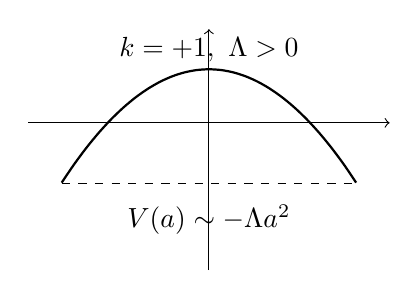
\begin{tikzpicture}[scale=0.85]
\draw[->] (-2.7,0) -- (2.7,0);
\draw[->] (0,-2.2) -- (0,1.4);
\draw[thick,domain=-2.2:2.2,smooth] plot (\x,{-0.35*(\x)^2 + 0.8});
\draw[dashed] (-2.2,-0.9) -- (2.2,-0.9);
\node at (0,-1.45) {\(V(a)\sim -\Lambda a^2\)};
\node at (0,1.1) {\(k=+1,\ \Lambda>0\)};
\end{tikzpicture}
\hspace{2em}
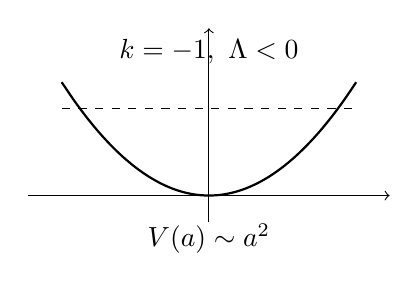
\begin{tikzpicture}[scale=0.85]
\draw[->] (-2.7,0) -- (2.7,0);
\draw[->] (0,-0.4) -- (0,2.5);
\draw[thick,domain=-2.2:2.2,smooth] plot (\x,{0.35*(\x)^2});
\draw[dashed] (-2.2,1.3) -- (2.2,1.3);
\node at (0,-0.65) {\(V(a)\sim a^2\)};
\node at (0,2.15) {\(k=-1,\ \Lambda<0\)};
\end{tikzpicture}
\caption{Transcript-backed schematic potentials for the mechanical analogies used in the lecture.}
\end{figure}

These examples carry the methodological lesson that closes the lecture's main development: many Friedmann equations can be understood by translating cosmology into the mechanics of a fictitious particle moving in an effective potential.

\section{Summary}

The lecture begins with the familiar question of how \(a(t)\) evolves and then isolates the missing input: the equation of state. From the thermodynamic box argument we obtain the general density law
\[
\rho\propto a^{-3(1+w)}.
\]
Matter then gives \(w=0\) and \(\rho\propto a^{-3}\), while radiation gives \(w=\tfrac13\) and \(\rho\propto a^{-4}\). The radiation result is not taken on faith; it is derived from photon momentum transfer and the isotropic average \(\langle \cos^2\theta\rangle=\tfrac13\).

The second half of the lecture shifts to negative pressure. Tension provides the intuition, vacuum energy provides the cosmological realization, and the backward box argument gives \(w=-1\). Once that equation of state is in hand, the Friedmann equation yields exponential de Sitter expansion for flat positive \(\Lambda\), a bounce-like \(\cosh\) solution for \(k=+1\) and positive \(\Lambda\), and re-collapse for \(k=-1\) with negative \(\Lambda\). The final perspective is equally important: the existence of vacuum energy is not the deepest surprise. The surprise is how extraordinarily small it is.